\section{Results}

Results of the experiment support our theory that the tested models use distance features.

\subsection{Baseline Performance}


Both models achieved strong classification performance on MNIST before perturbation testing, as shown in Table~\ref{tab:baseline}.

\begin{table}[h]
\centering
\begin{tabular}{lrrr}
\hline
Model & Training Acc (\%) & Test Acc (\%) & Loss \\
\hline
PerturbationAbs & 99.99 $\pm$ 0.00 & 95.29 $\pm$ 0.20 & 0.0047 $\pm$ 0.0005 \\
PerturbationReLU & 98.33 $\pm$ 0.15 & 95.61 $\pm$ 0.14 & 0.0610 $\pm$ 0.0044 \\
\hline
\end{tabular}
\caption{Baseline model performance averaged across 20 training runs (mean $\pm$ standard deviation).}
\label{tab:baseline}
\end{table}

\subsection{Perturbation Analysis}

Both models demonstrate strong invariance to intensity scaling while showing significant sensitivity to distance perturbations, supporting our theoretical framework. Figure~\ref{fig:perturbation_analysis} shows these effects across both perturbation types.

The PerturbationAbs model maintains consistent performance across a wide range of intensity scales while showing dramatic accuracy degradation under distance perturbations, dropping to 11.80\% accuracy at 0.4 offset. The PerturbationReLU model exhibits similar patterns, though with more moderate effects, maintaining 50.99\% accuracy at the same offset.

\begin{figure}[h]
    \centering
    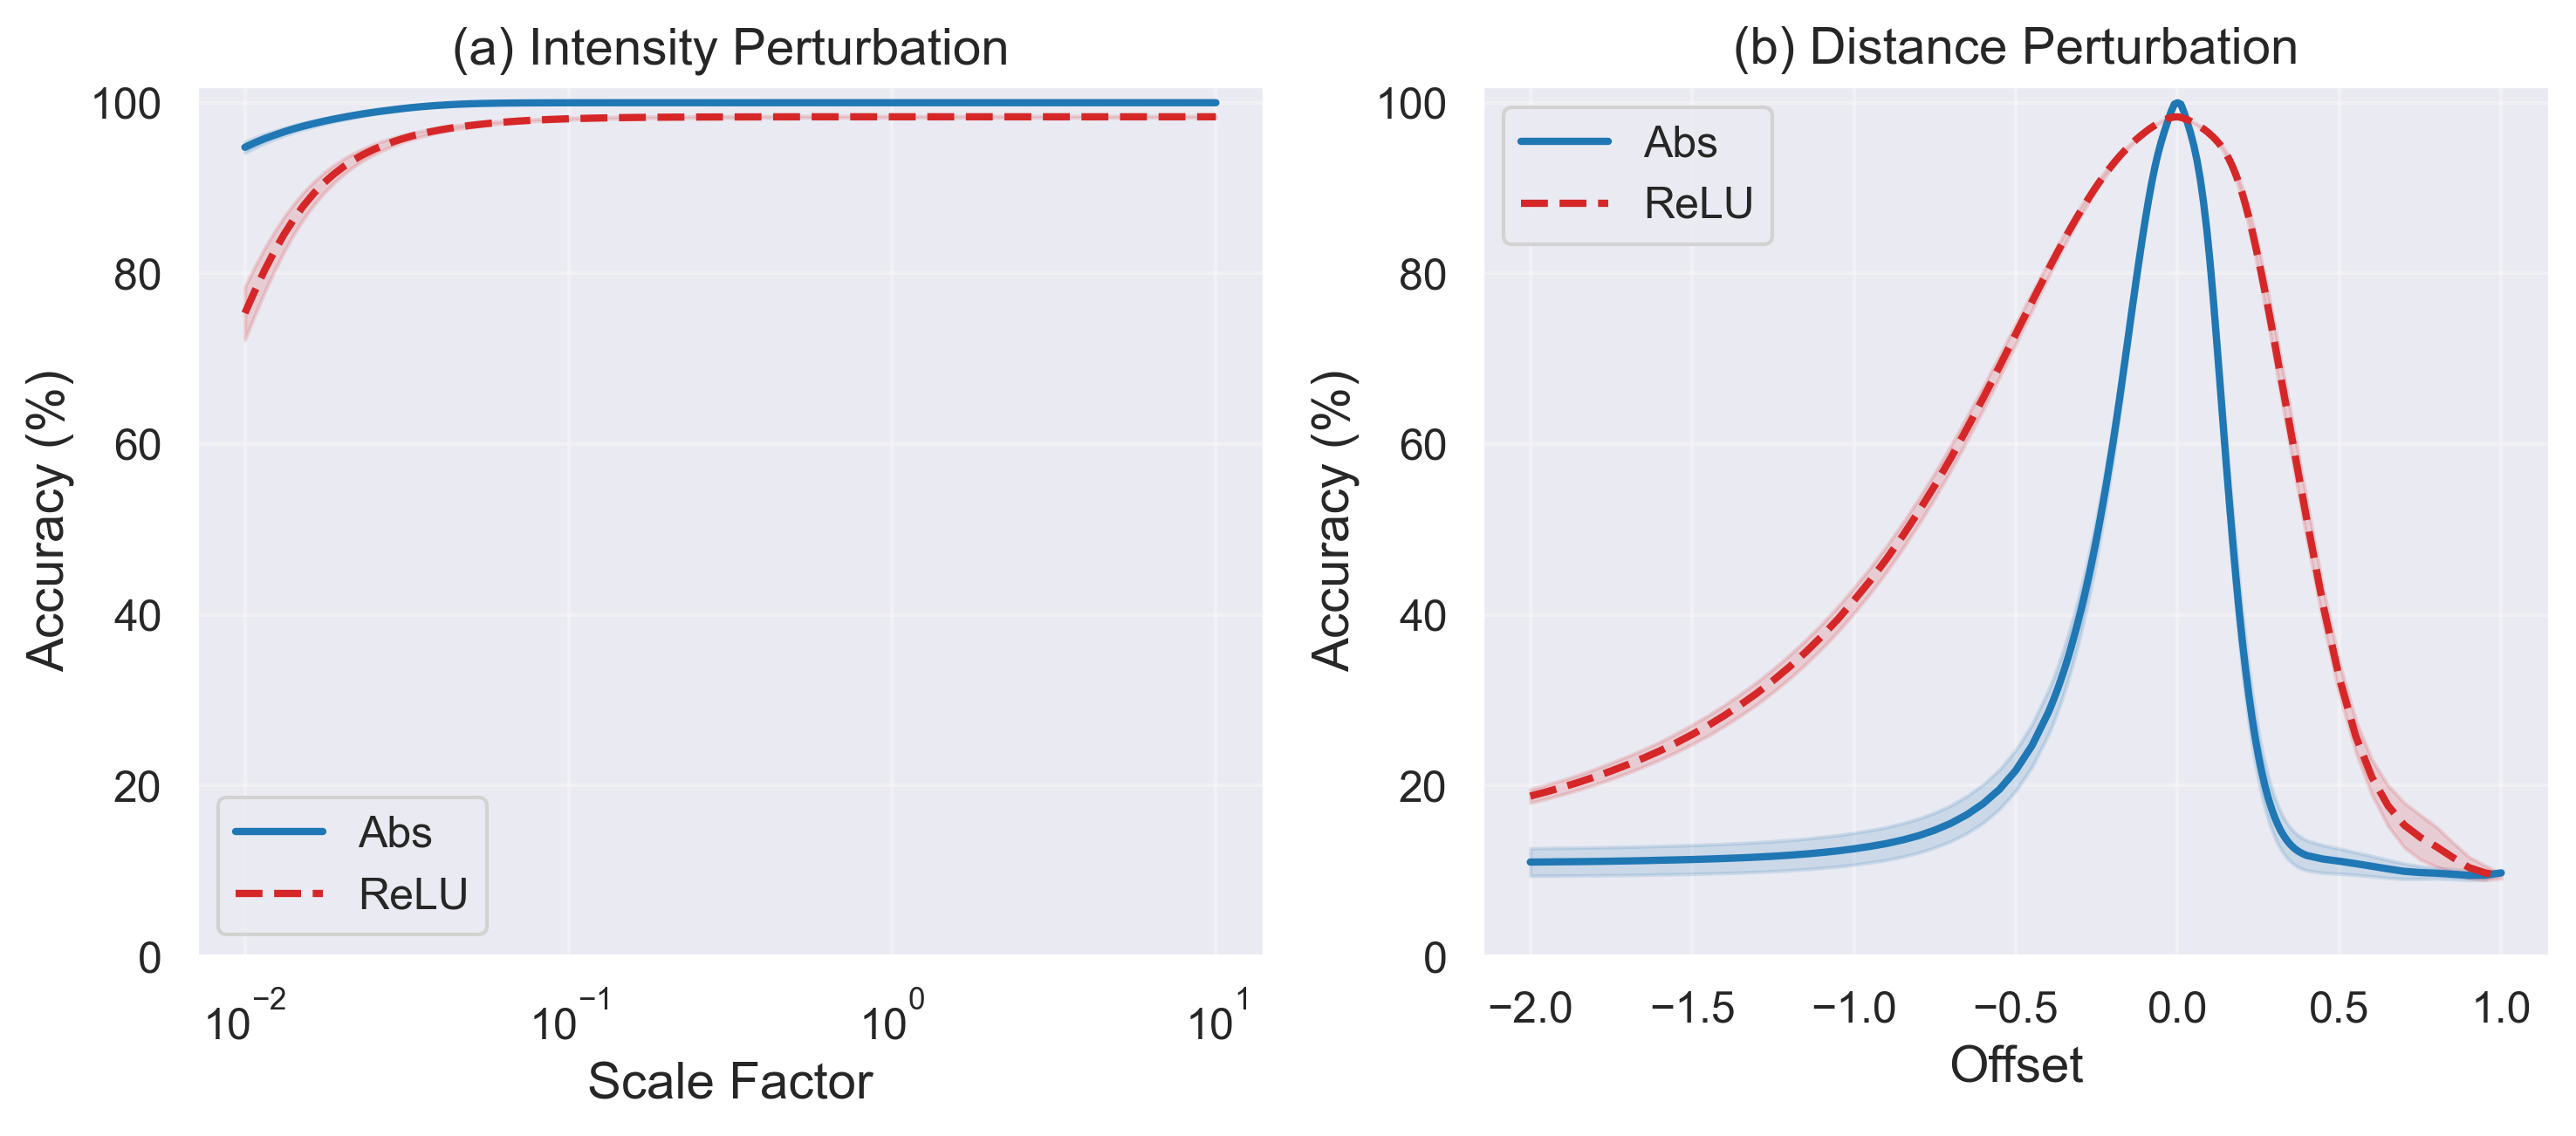
\includegraphics[width=\textwidth]{images/perturbation_analysis}
    \caption{Effects of intensity scaling and distance offset perturbations on model accuracy. Shaded regions represent 95\% confidence intervals across 20 runs.}
    \label{fig:perturbation_analysis}
    \end{figure}
\subsection{Statistical Analysis}

Table~\ref{tab:ttest} shows the statistical significance of these effects through paired t-tests comparing perturbed performance against baseline accuracy. Both models show highly significant responses to distance perturbations ($p < 10^{-16}$), while only the PerturbationReLU model shows modest sensitivity to intensity scaling ($p < 0.005$).

\begin{table}[h]
\centering
\begin{tabular}{llrrr}
\hline
Model & Test & T-statistic & P-value & Mean Acc (\%) \\
\hline
\multirow{4}{*}{PerturbationAbs} 
 & Scale 0.5 & -2.031 & 5.645e-02 & 99.99 \\
 & Scale 2.0 & -2.015 & 5.829e-02 & 99.99 \\
 & Offset -0.4 & 41.305 & 4.545e-20 & 28.51 \\
 & Offset 0.4 & 26.519 & 1.790e-16 & 11.80 \\
\hline
\multirow{4}{*}{PerturbationReLU}
 & Scale 0.5 & -3.689 & 1.558e-03 & 98.33 \\
 & Scale 2.0 & -3.202 & 4.693e-03 & 98.33 \\
 & Offset -0.4 & 40.709 & 5.973e-20 & 80.38 \\
 & Offset 0.4 & 37.155 & 3.319e-19 & 50.99 \\
\hline
\end{tabular}
\caption{Statistical significance of perturbation effects compared to baseline performance.}
\label{tab:ttest}
\end{table}

We observe a transition point in the intensity perturbation results around scale factor 0.08, where both models begin to show degraded performance. We believe this represents the scale at which intensity-based activations approach the magnitude range where distance-based features typically operate.